% This is samplepaper.tex, a sample chapter demonstrating the
% LLNCS macro package for Springer Computer Science proceedings;
% Version 2.20 of 2017/10/04
%
\documentclass[runningheads]{llncs}
%
\usepackage{graphicx}
\usepackage{float}
\usepackage{subcaption}
\captionsetup{compatibility=false}

% Used for displaying a sample figure. If possible, figure files should
% be included in EPS format.
%
% If you use the hyperref package, please uncomment the following line
% to display URLs in blue roman font according to Springer's eBook style:
% \renewcommand\UrlFont{\color{blue}\rmfamily}

\begin{document}
%
\title{Bachelor Dissertation}
%
%\titlerunning{Abbreviated paper title}
% If the paper title is too long for the running head, you can set
% an abbreviated paper title here
%
\author{Kasper Engelen\and
		Jonathan Meyer\and
		Dawid Miroyan\and
		Igor Schittekat}
%
%
\institute{University of Antwerp}
%
\maketitle              % typeset the header of the contribution
%
\begin{abstract}
This document reports our findings regarding the final dissertation. The sections and subsections correspond to the assignments given to us. In this project we worked with a simulator called Stride, developed at the University of Antwerp. We explore various concepts within computational epidemiology through the use of this program. 

\keywords{Computational Epidemiology  \and Dissertation}
\end{abstract}
%
%
%
\section{Simulation}
\subsection{Stochastic Variation}

\paragraph{} The first topic we consider is stochastic variation. Since the simulation uses a pseudo-random number generator, it's useful to inspect the influence of this stochasticity on the results of the simulation. Using the Stan tool which is provided with Stride, we collected data on 100 simulations with an identical configuration file. The only difference between executions is the RNG seed. When plotting the results, it becomes apparent that the amount of new cases per day follows a normal distribution. For the data we collected, we calculated a  mean of 33.33 new cases per day, and a variance of 1196.99. Looking at the plot for the cumulative cases per day, two 'categories' can be distinguished:  'outbreak' scenarios and 'extinction' scenarios. These cases are quite evenly spread, which explains the high variance for new cases per day. In the former, the curve has a sigmoid shape, indicating that the disease succesfully spread among the population. The latter scenario corresponds to the curves that are almost constant and are bounded by a value well under the population size. In these cases, the disease did not manage to spread, resulting in only a few infected people at the end of the simulation. This is likely explained by the initial infectation: if the first person to be infected is sufficiently isolated (either socially or by being surrounded by people who are immune), the disease doesn't have a chance to spread.\\
Figure \ref{casesPlots} shows the different scenarios. In the cumulative cases plot the 'extinction' senario is clearly visible at the bottom. The plot for new cases per day is very jagged, which can also be explained by the stochastic nature of the simulation.

\begin{figure}[h!]
	\centering
	\begin{subfigure}[b]{0.7\linewidth}
		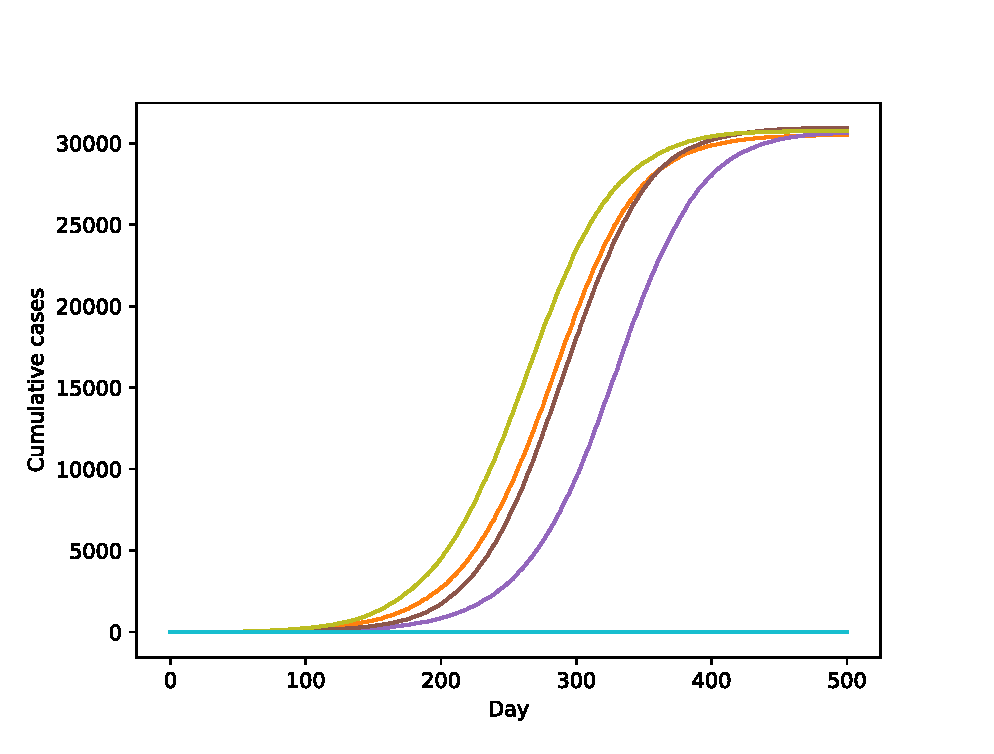
\includegraphics[width=\linewidth]{cases_cum.eps}
		\caption{Cumulative cases per day.}
	\end{subfigure}
	\begin{subfigure}[b]{0.7\linewidth}
		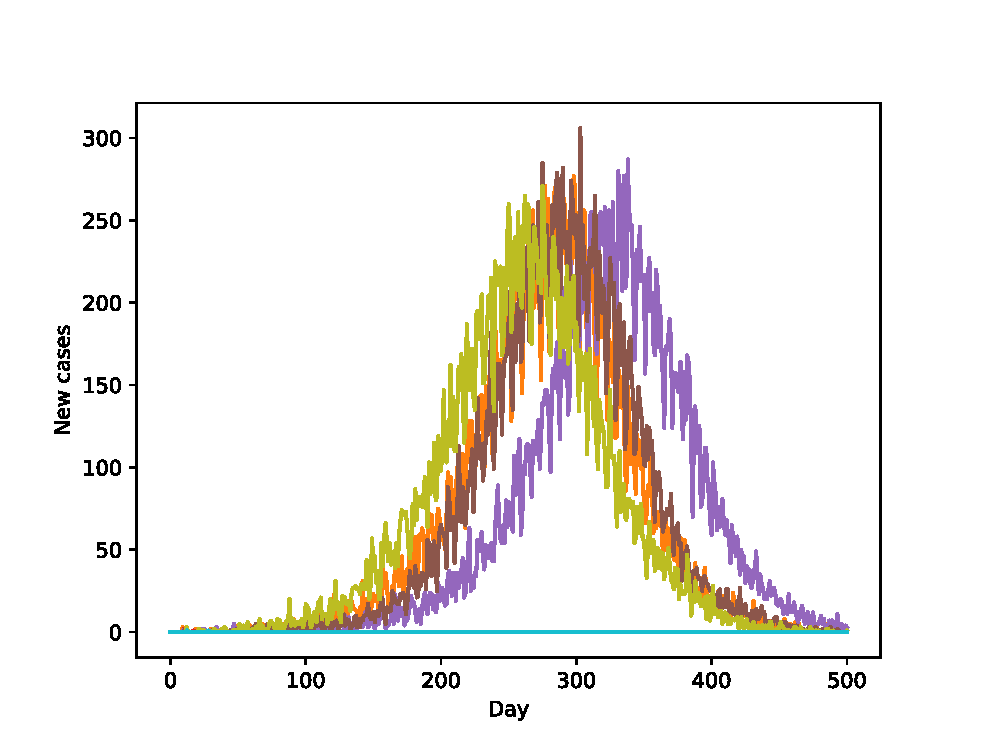
\includegraphics[width=\linewidth]{cases_per_day.eps}
		\caption{New cases per day.}
	\end{subfigure}
	\caption{Results of five different simulations, using the configuration file \emph{stochastic\_analysis.xml}}
	\label{casesPlots}
\end{figure}


\subsection{Extinction Threshold}

\paragraph{} As discussed previously, it might be the case that only very few people become infected over the course of a simulation. This is referred to as extinction. There is a clear distinction between outbreaks and extinctions, so in this subsection we attempt to find an \emph{extinction threshold}.

\paragraph{} Figure \ref{ETHist} gives the frequencies of the amount of infected people at the end of the simulations. The distinction between outbreaks and extinctions is quite clear from this histogram. There is one peak on the lower end of the x-axis, and there is a cluster on the higher-end. It is hard to find a good concrete value for the threshold, but the total amount of infected people in an extinction is always significantly under the total population size. Therefore, a fraction of the total population could be used as treshold. In our simulations the amount of cases after extinction never exceeded 50, so a threshold of 0.01\% of the population seems reasonable.

\begin{figure}[!h]
	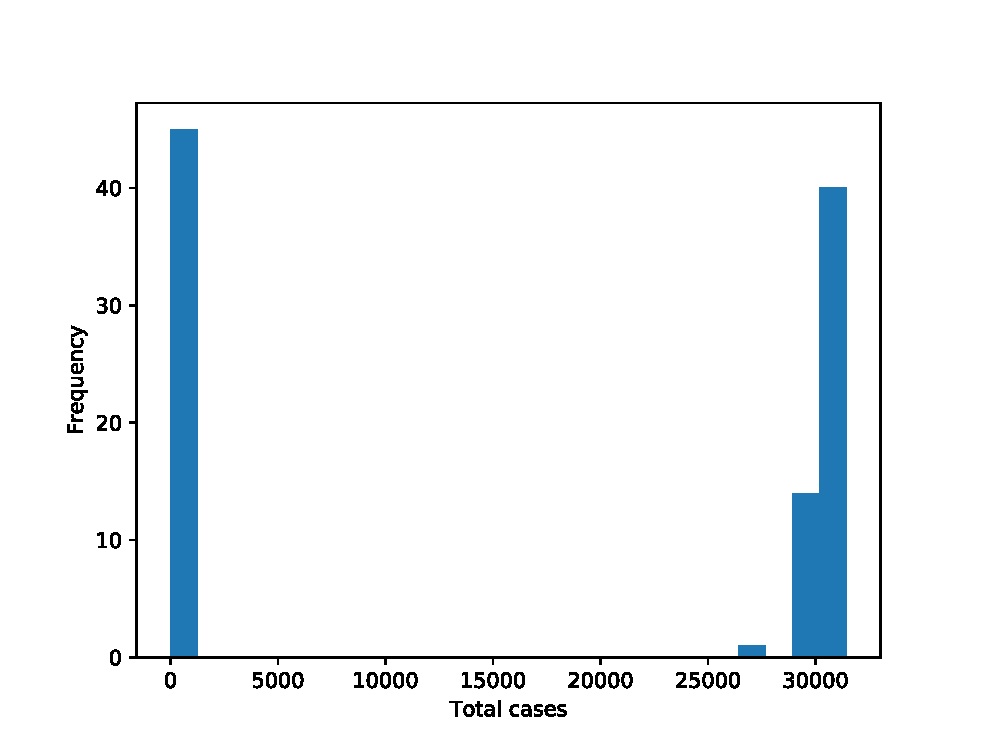
\includegraphics[width=\textwidth]{Hist.eps}
	\caption{Frequencies of final amounts of cases for 100 simulations.} 
	\label{ETHist}
\end{figure}

\subsection{Immunity Level}

\paragraph{} In order to make assumptions about the population's immunity level, we look at the simulated results for different values. Upon experimentation, it becomes apparent the immunity level is approximately 70\% of the population. Figure \ref{immLvlPlot} shows the average new cases per day for different immunity levels. The reference curve is also included. This plot was generated by taking the average of new cases per day over 20 simulations per immunity level. Using PyStride to simulate outbreaks, we narrowed down the immunity level $I$ to \( 0.705 \leq I \leq 0.7175 \).

\begin{figure}[H]
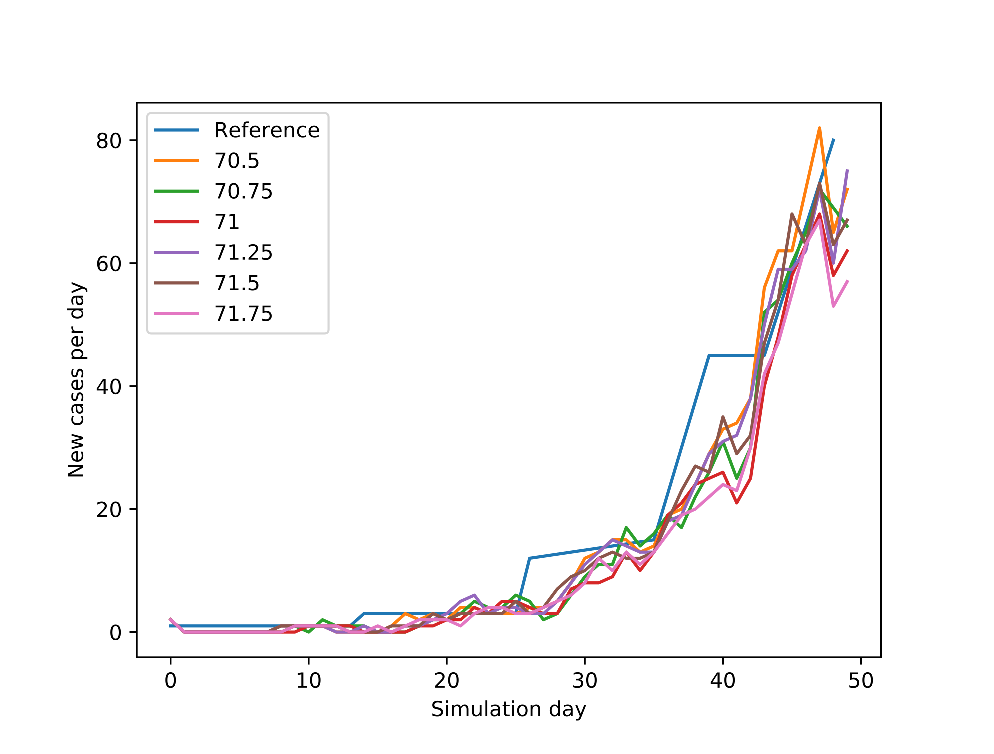
\includegraphics[width=\textwidth]{ImmLvl.eps}
\caption{Average new cases per day, calculated from 20 simulations per immunity level.} 
\label{immLvlPlot}
\end{figure}


\subsection{Estimating $R_{0}$}

\paragraph{} Now that we have a relatively decent estimate for the immunity level of the population, we can do an analogous exercise to estimate $R_0$. For this data, we fixed the immunity level to 70.5\%. Figure \ref{R0EstPlot} (a) shows the plot for each possible $R_0$ in the range $[12, 18]$ (average over 20 simulations). It's clear that the best candidates are 14, 15 or potentially 16. When we plot a more detailed plot for just those valued (average over 30 different simulations), it seems 15 is the best estimate for $R_0$.

\begin{figure}[H]
	\centering
	\begin{subfigure}[b]{0.7\linewidth}
		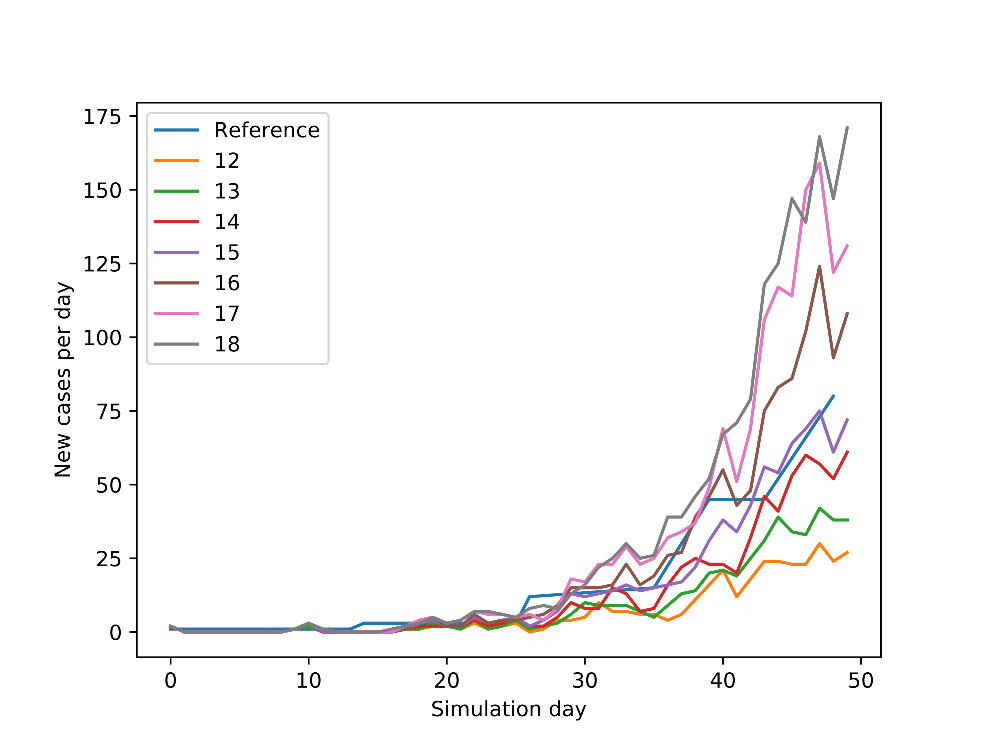
\includegraphics[width=\textwidth]{R0_all_20runs.eps}
		\caption{Overview of all potential $R_0$'s. Averages from 20 runs per $R_0$.} 	
	\end{subfigure}
	\begin{subfigure}[b]{0.7\linewidth}
		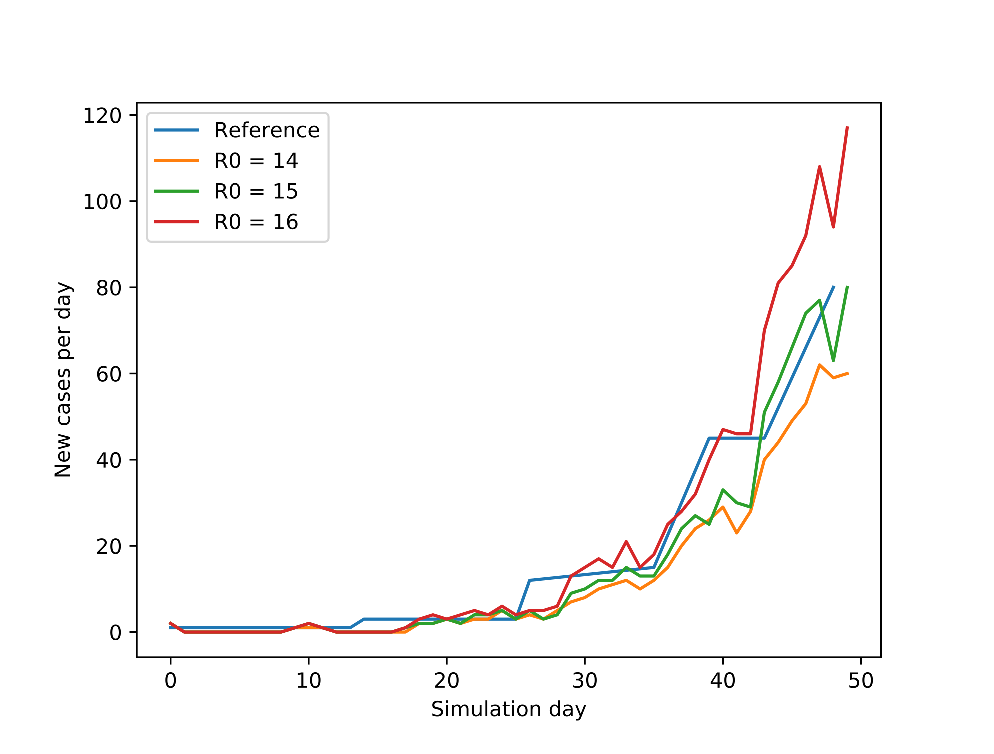
\includegraphics[width=\textwidth]{R0_detail_30runs.eps}
		\caption{More detailed look at $R_0$ candidates. Averages from 30 runs per $R_0$.} 
	\end{subfigure}
	\caption{Averages for different values of $R_0$.}
	\label{R0EstPlot}
\end{figure}

\section{Population generation}

\subsection{Influence of demography}

% outbreak risico, outbreak grootte
\paragraph{} We want to test whether or not the age distribution of a population has an influence on the size and probability of an outbreak. To do this we have two populations, namely region A and region B and we sample households from these two populations. 

\begin{figure}[H]
\centering
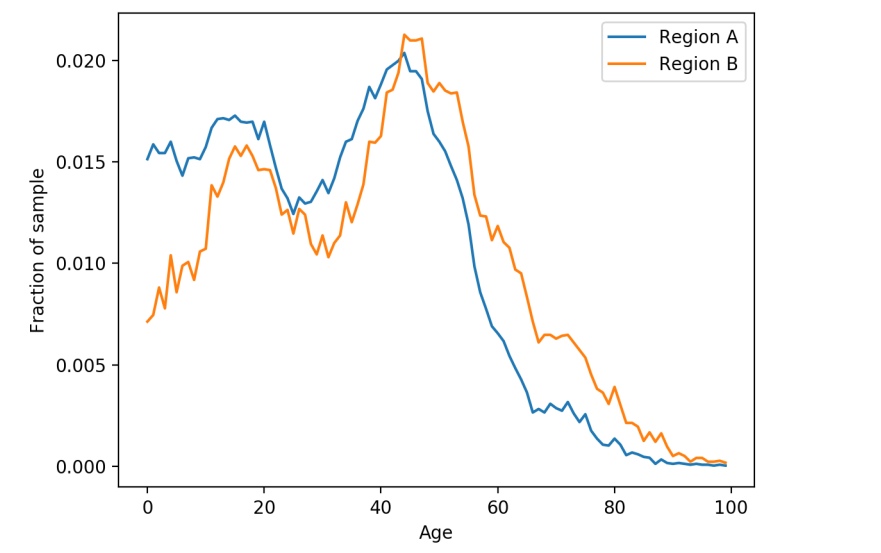
\includegraphics[width=0.8\textwidth]{./2_1_regionDiff/plot_ageDistr.png}
\caption{The age distribution of region A and region B.}
\label{2_1_regionDiff_plotAgeDistr}
\end{figure}

\paragraph{} We determined a large number of sets of parameters and ran simulations using these parameters. By using statistics and plots of the obtained data we determined 6 sets of interesting parameters:

%%parameters
\begin{table}[H]
\centering
\begin{tabular}{|l|l|l|}
\hline
\textbf{Region} & \textbf{Seeding rate} & \textbf{Number of days} \\
\hline
Region A & 0.002      & 50 \\
\hline
Region A & 0.002      & 300 \\
\hline
Region A & 0.00000167 & 300 \\
\hline
Region B & 0.002      & 50 \\
\hline
Region B & 0.002      & 300 \\
\hline
Region B & 0.00000167 & 300 \\
\hline
\end{tabular}
\caption{The different parameter sets that we found to be interesting.}
\label{2_1_regionDiff_tableParamSets}
\end{table}

% verschillende parameters toelichten

\paragraph{} All the simulations started on the 11th of March 2019, with $R_0$ equal to $11$ and a randomized vaccination policy with a rate of $0.8$. \textit{Seeding rate} here means the fraction of the population that is initially infected.

\paragraph{} Once we determined which simulation parameters are interesting, we ran 1000 simulations with each set of parameters.

\subsubsection{Comparing outbreak sizes}

\paragraph{} Before analyzing the outbreak sizes, we first filtered out all the simulations that did not lead to an outbreak. For the simulations with seeding rate equal to $0.002$ the \textit{extinction threshold} was taken to be $5000$, for seeding rate equal to $0.00000167$ we used $40000$. One should note that when setting seeding rate to $0.002$ there was a 100\% outbreak rate and as such filtering out the extinctions was not really necessary.


\begin{figure}[H]
\centering

\begin{subfigure}[b]{0.7\linewidth}
% RegionAvsB, SR=0.002,      Days=50
\includegraphics[width=\textwidth]{./2_1_regionDiff/{plot_compSize_SR=0.002_Days=50_FINALDAY_HIST}.eps}
\caption{Plot for simulation over 50 days with seeding rate $0.02$.}
\end{subfigure}

\begin{subfigure}[b]{0.7\linewidth}
% RegionAvsB, SR=0.002,      Days=300
\includegraphics[width=\textwidth]{./2_1_regionDiff/{plot_compSize_SR=0.002_Days=300_FINALDAY_HIST}.eps}
\caption{Plot for simulation over 300 days with seeding rate $0.02$.}
\end{subfigure}

\begin{subfigure}[b]{0.7\linewidth}
% RegionAvsB, SR=0.00000167, Days=300
\includegraphics[width=\textwidth]{./2_1_regionDiff/{plot_compSize_SR=0.00000167_Days=300_FINALDAY_HIST}.eps}
\caption{Plot for simulation over 300 days with seeding rate $0.00000167$.}
\end{subfigure}
\caption{Plots that compare the outbreak sizes of region A and region B using different parameters.}
\end{figure}

\subsubsection{Comparing outbreak rates}

\paragraph{} In order to analyze the outbreak rate, we only looked at the simulations with seeding rate equal to $0.00000167$, since with seeding rate equal to $0.002$ there was a 100\% outbreak rate. The following plot contains a histogram that depics the amount of infected individuals in the different simulations.

% figure
\begin{figure}[H]
\centering
\includegraphics[width=0.8\textwidth]{./2_1_regionDiff/{plot_compRate_SR=0.00000167_Days=300_FINALDAY_HIST}.eps}
\end{figure}

\paragraph{} We can see that there is a difference between region A and region B which leads to region A having a higher outbreak rate than region B. We also determined a 95\% confidence interval for the outbreak probability of region A:

$$ [77.625\%, 82.575\%] $$

\paragraph{} As well as an interval of the same confidence for region B:

$$ [73.561\%, 78.839\%] $$

\paragraph{} We can clearly see that the outbreak rate of region A lies higher than that of region B.

\subsection{Vaccinating on campus}

\paragraph{} By vaccinating the students, quickly after infected individuals appear in the population, we want to test whether so called 'catch-up' campaigns have a noticeable impact on an outbreak. \\
For these simulations, we generated a population where 60\% of people between the age of 18 and 26 attend high education. We then simulate scenarios where all students are either vaccinated on day 7 or not vaccinated at all. When looking at Figure \ref{VaccinePlot}, the amount of new cases is the same in both scenarios on day 5 and 6. As the students are not vaccinated in both scenarios, some of them become infected and can spread the disease. Starting from day 7, where in one of the scenarios the susceptible students are vaccinated, the amount of new cases is lower than when not vaccinating.

\begin{figure}[h!]
	\centering
	\begin{subfigure}[b]{0.7\linewidth}
		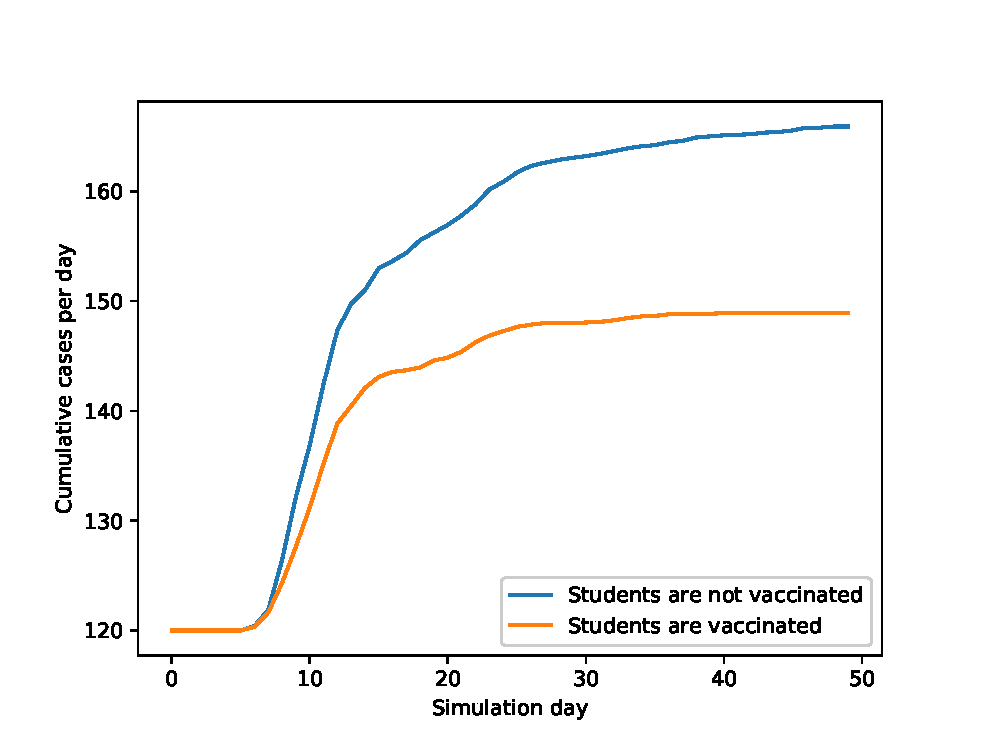
\includegraphics[width=\textwidth]{vaccinating_cases_cum_20runs.eps}
		\caption{Plot showing the amount of infected student per day.} 	
	\end{subfigure}
	\begin{subfigure}[b]{0.7\linewidth}
		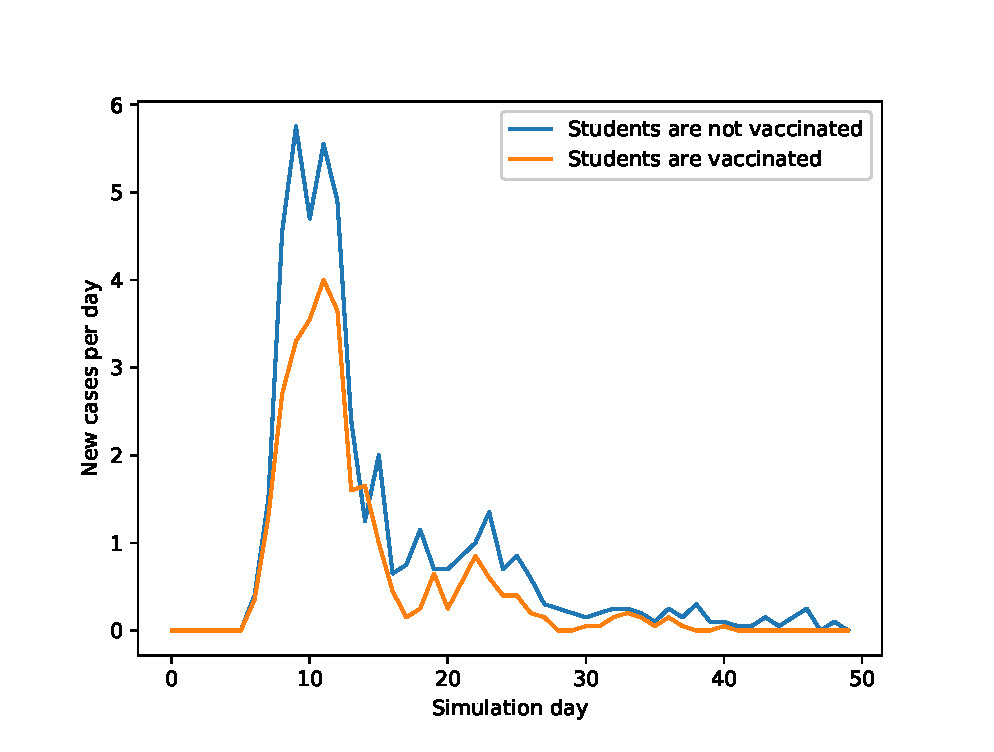
\includegraphics[width=\textwidth]{vaccinating_cases_per_day_20runs.eps}
		\caption{Plot showing the amount of newly infected student per day.} 
	\end{subfigure}
	\caption{Plots showing the impact of vaccinating students. Averages from 20 simulations.}
	\label{VaccinePlot}
\end{figure}

\newpage

\subsection{Commuting to work}

\paragraph{} Another factor that is interesting to examine is the impact of commuting on disease spread. \\
In this simulation, we generate different populations, depending on different fractions of commuters. The expectation we have is that if more people commute to work, more people gets infected in the end. But when we run the simulation, we see that there isn't a difference between the fraction of commuters. We can also see that there is a peak between day 40 and 50. This peak doesn't change much when we increase the amount of commuters. If we increase the amount of days to 200, the peak is around 70-75, but still no difference between the fractions of commuters. 

\begin{figure}[h!]
	\centering
	\begin{subfigure}[b]{0.7\linewidth}
		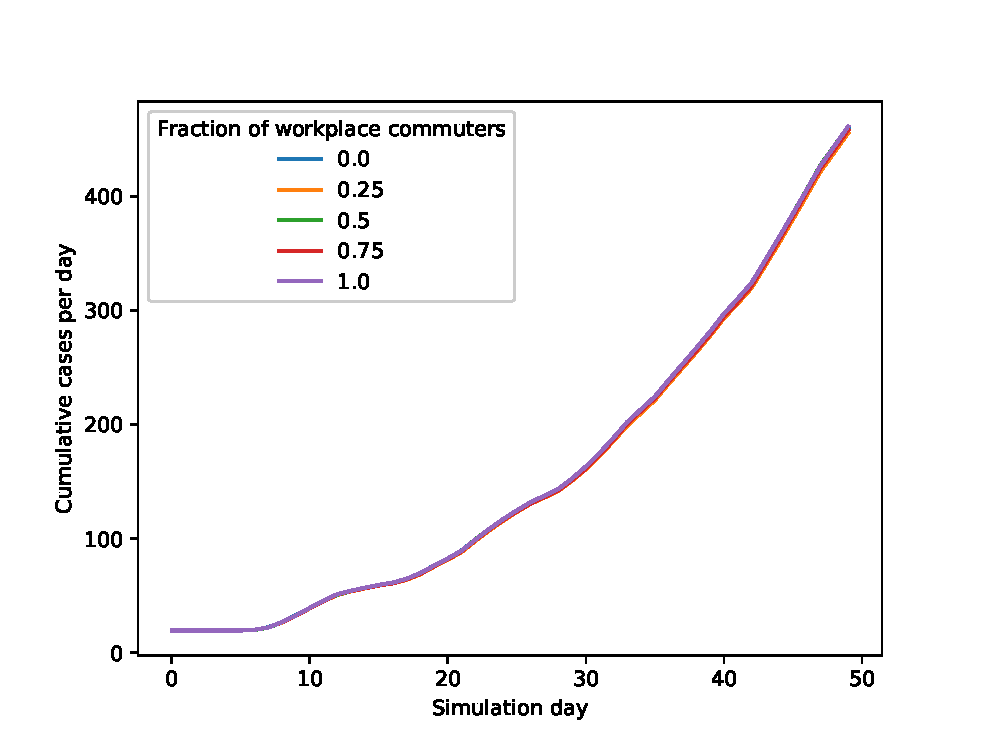
\includegraphics[width=\textwidth]{work_cum_1.eps}
		\caption{Cumulative cases per day} 
	\end{subfigure}
	\begin{subfigure}[b]{0.7\linewidth}
		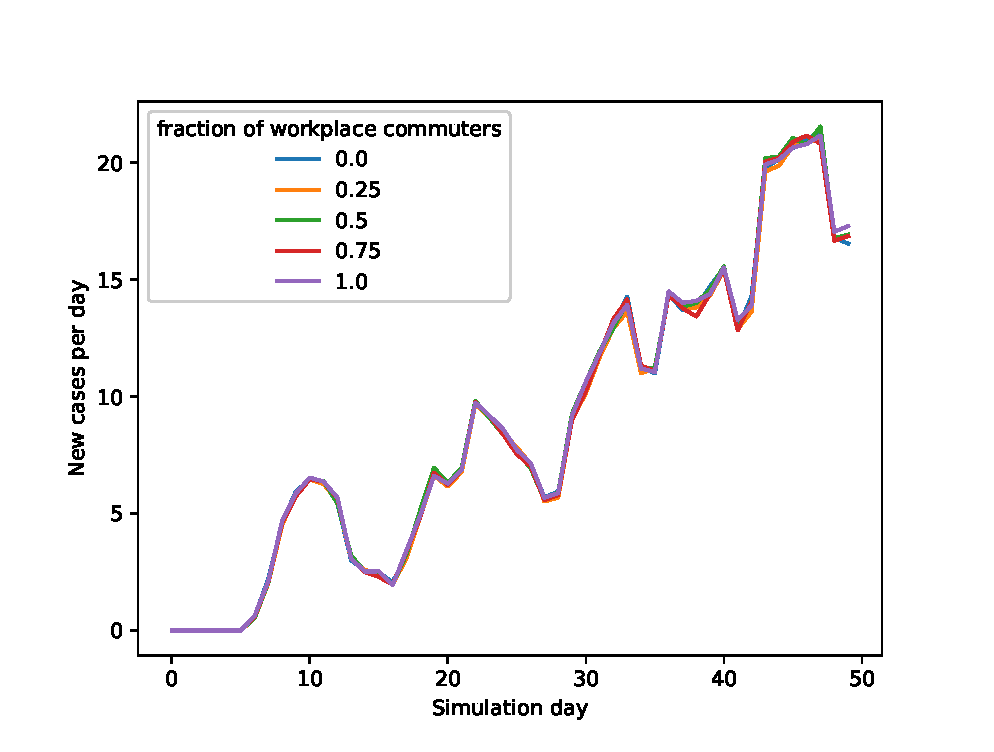
\includegraphics[width=\textwidth]{work_cases_per_day_1.eps}
		\caption{New cases per day.} 
	\end{subfigure}
	\caption{Plots showing the impact of Commuting to work on a population of size 10000. 1000 runs for each fraction. }
	\label{VaccinePlot}
\end{figure}

\begin{figure}[h!]
	\centering
	\begin{subfigure}[b]{0.7\linewidth}
		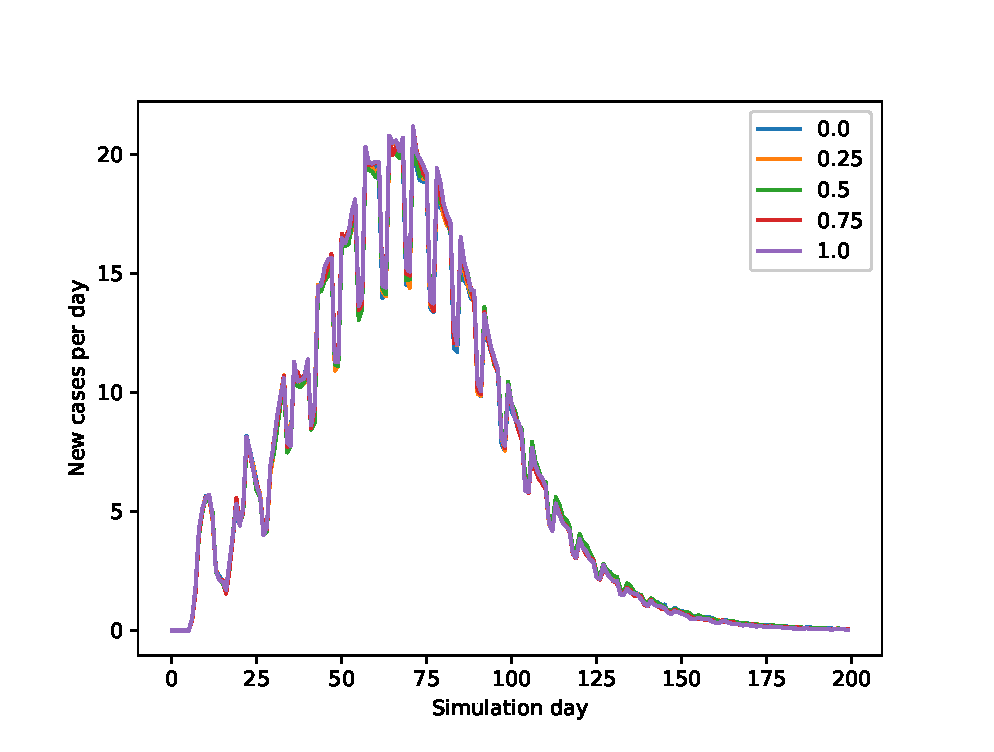
\includegraphics[width=\textwidth]{work_cases_per_day_3.eps}
		\caption{New cases per day.} 
	\end{subfigure}
	\caption{Plots showing the impact of Commuting to work on a population of size 10000. 1000 runs for each fraction. 200 days.}
	\label{VaccinePlot}
\end{figure}

\newpage
When we increase the population size, we don't see many differences. 

\begin{figure}[h!]
	\centering
	\begin{subfigure}[b]{0.7\linewidth}
		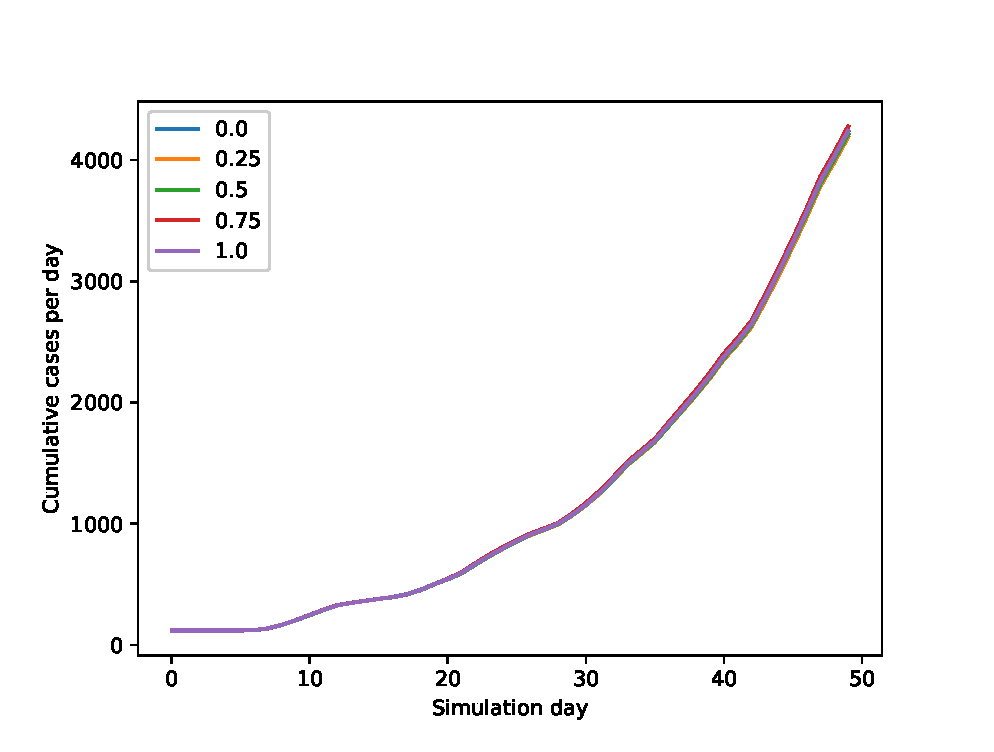
\includegraphics[width=\textwidth]{work_cum_2.eps}
		\caption{Cumulative cases per day} 
	\end{subfigure}
	\begin{subfigure}[b]{0.7\linewidth}
		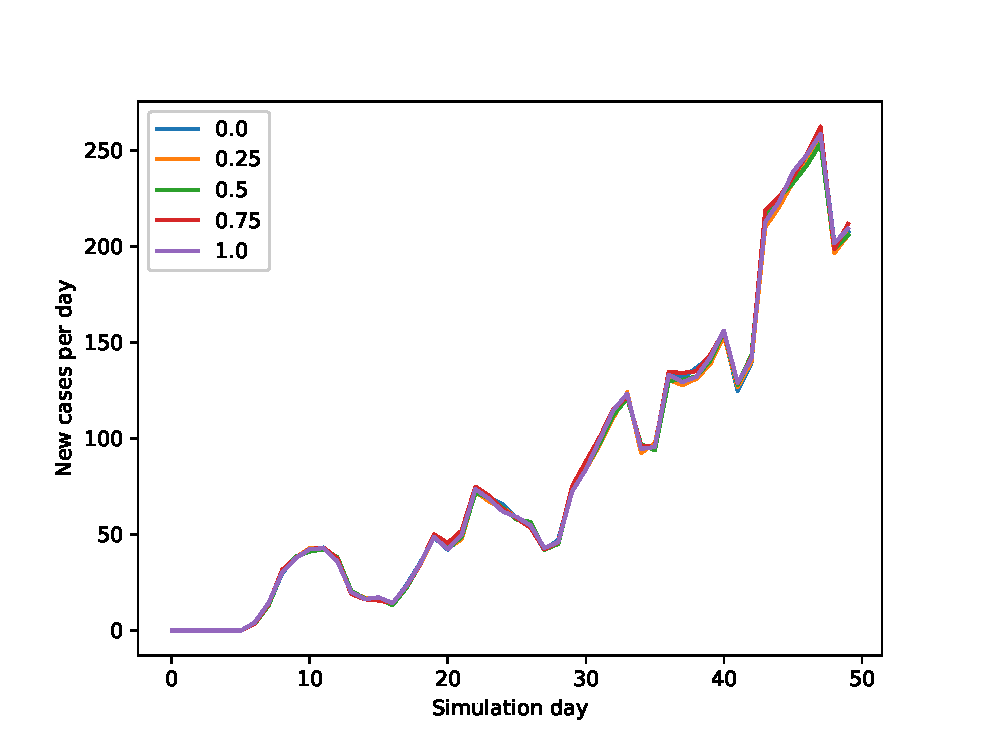
\includegraphics[width=\textwidth]{work_cases_per_day_2.eps}
		\caption{Plots showing the impact of Commuting to work on a population of size 600000. 100 runs for each fraction. } 
	\end{subfigure}
	\caption{Plots showing the impact of Commuting to work on a population of size 500000}
	\label{VaccinePlot}
\end{figure}

\clearpage
\section{Performance profiling}

\paragraph{} Using GProf, we will look at the performance in different scenarios. By varying parameters, we try to see which parts of the code they have an influence on, and which parts take up the most time. 
\\
For the first 4 parameters
\begin{itemize}
	\item amount of days
	\item population size
	\item immunity rate
	\item seeding rate
\end{itemize}
the actual sorting and analyzing of the population takes up most of the time.

\subsection{Number of days}

\paragraph{} By increasing the number of days to be simulated, the total execution time gets longer as well. This should be expected as more days means more times we simulate what goes on in a day.
\begin{figure}[h!]
\centering
	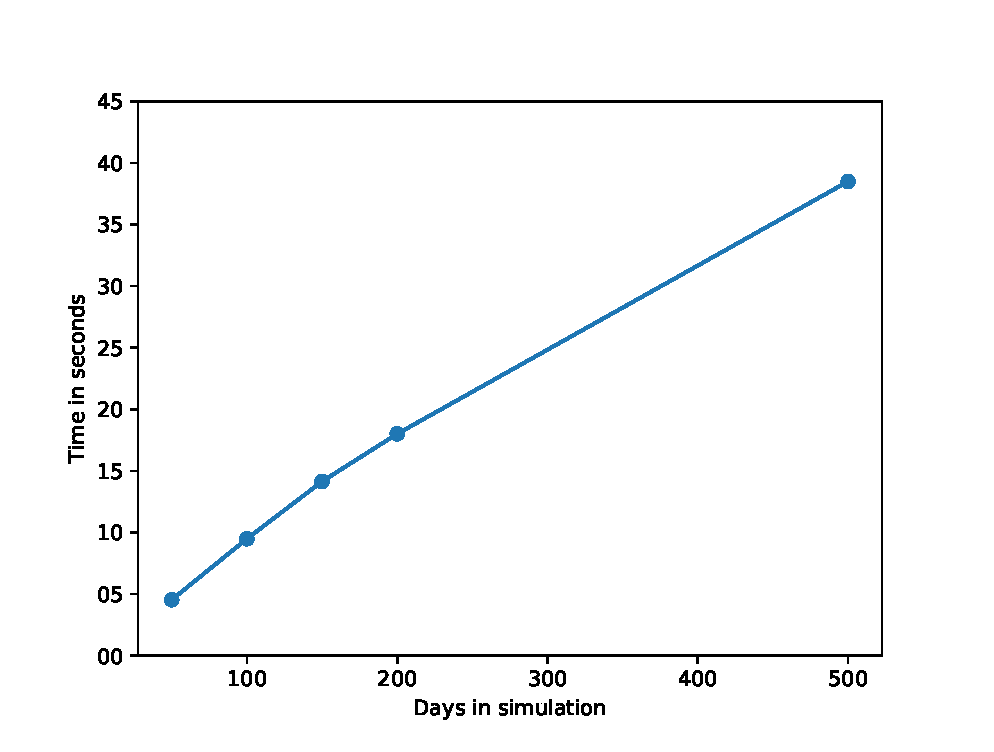
\includegraphics[width=0.8\textwidth]{3_GProf_numdays.eps}
	\caption{Plot showing run time of simulations by varying the number of days.} 
	\label{Gprof_numdays}
\end{figure}

\subsection{Population size}

\paragraph{} Generating a new population depends on the given size, which was expected. The generation however is very fast.
\begin{figure}[h!]
\centering
	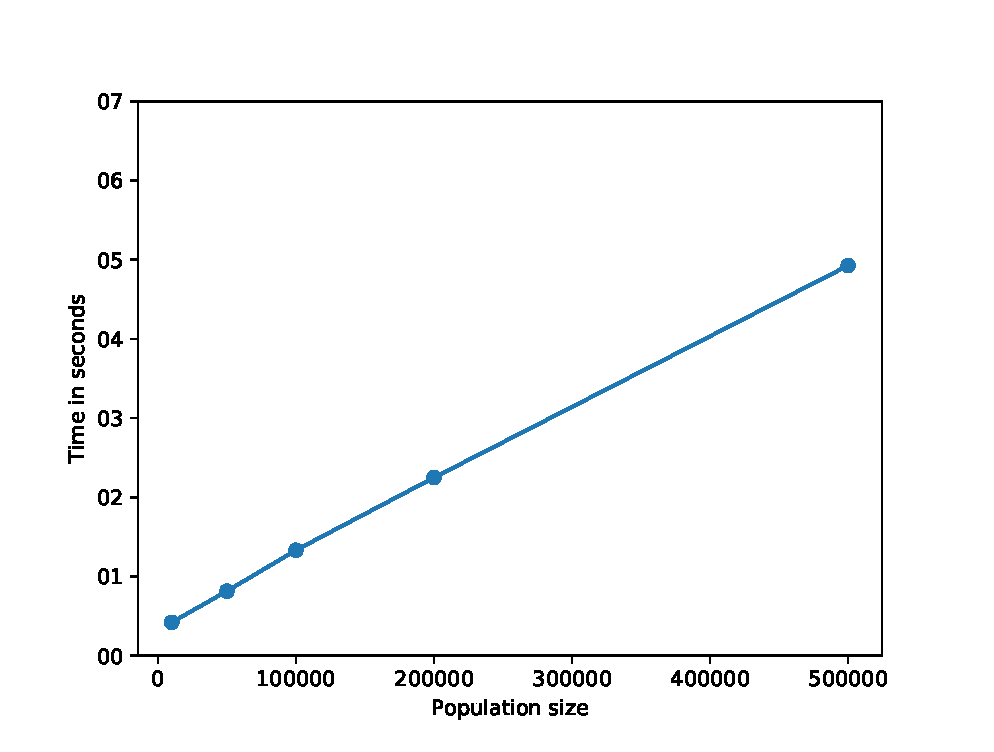
\includegraphics[width=0.8\textwidth]{3_GProf_popsize.eps}
	\caption{Plot showing run time of simulations by varying the size of the population.} 
	\label{Gprof_popsize}
\end{figure}

\subsection{Immunity rate}

\paragraph{} Varying the immunity rate does not seem to affect the total execution time.
\begin{figure}[h!]
\centering
	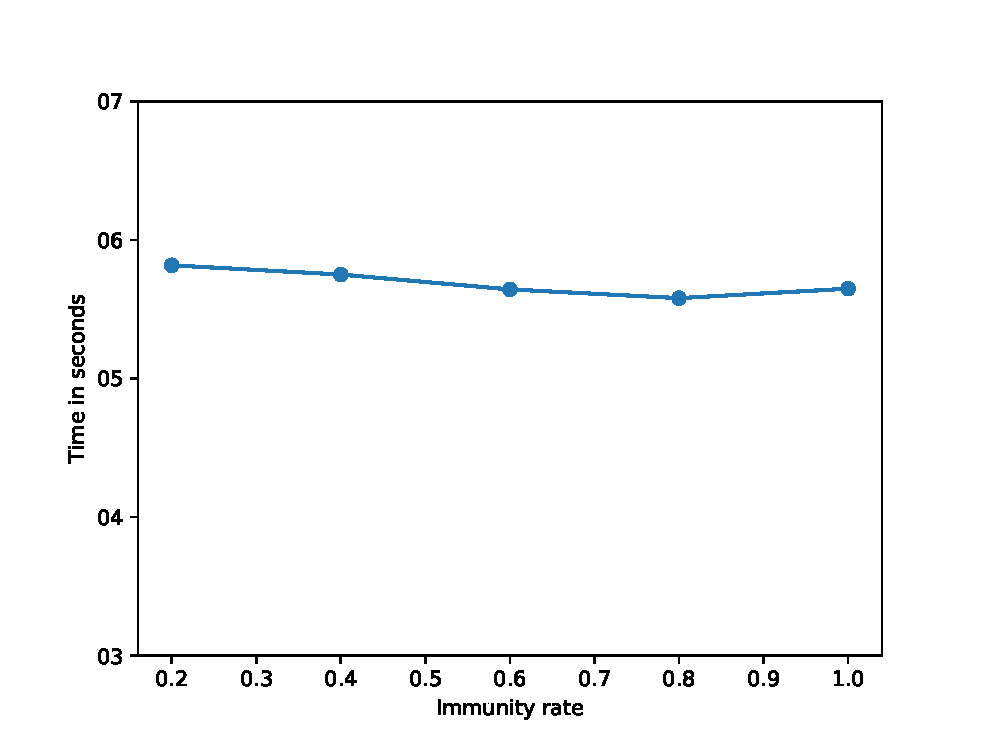
\includegraphics[width=0.8\textwidth]{3_GProf_immunityrate.eps}
	\caption{Plot showing run time of simulations by varying the immunity rate.} 
	\label{Gprof_immunityrate}
\end{figure}

\subsection{Seeding rate}

\paragraph{} A bigger seeding rate slightly increases the time of the execution. This happens as more people have to be initially infected.
\begin{figure}[h!]
\centering
	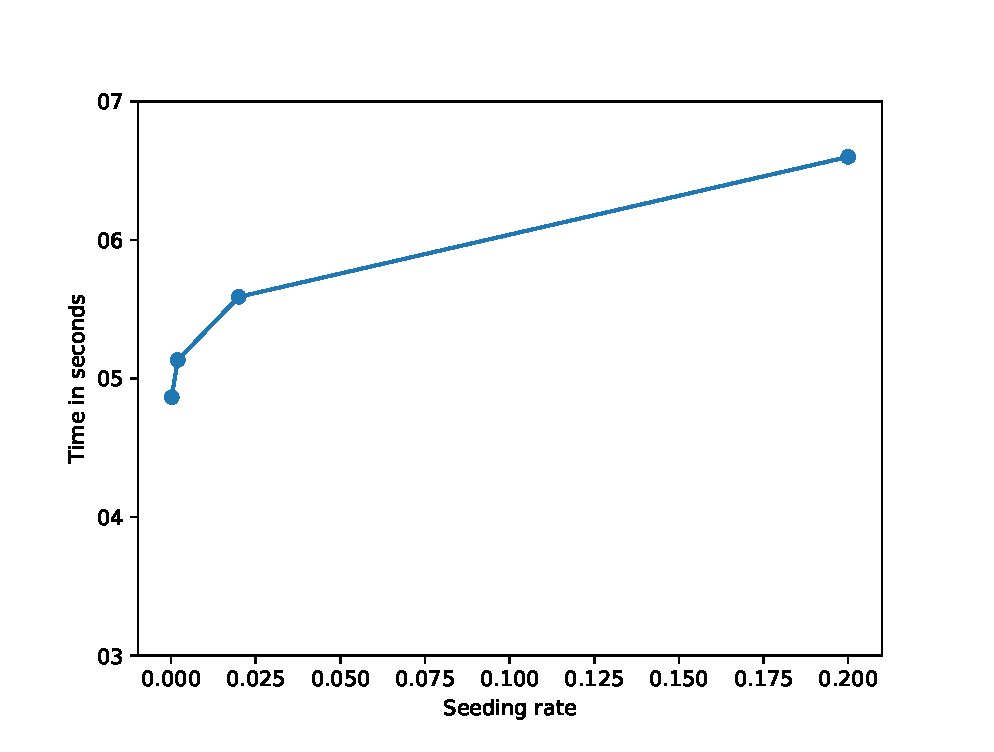
\includegraphics[width=0.8\textwidth]{3_GProf_seedingrate.eps}
	\caption{Plot showing run time of simulations by varying the seeding rate.} 
	\label{Gprof_seedingrate}
\end{figure}

\subsection{Contact log mode}

\paragraph{} The mode of the contact log has a very large impact on the execution time. Logging every contact between people takes a long time.\\
At day 50 in the simulation, only 20000 people out of 600000 where infected. When logging the susceptible people, you actually log almost 580000 people at each day which is very close to logging all people. This is very fast when the mode is set to Transmissions as you would only log once for each newly infected person. The logging modes 'All' and 'Susceptibles' use a less efficient algorithm, hence the big difference in run time between them and the modes 'Transmissions' and 'None'.\\

\begin{figure}[h!]
\centering
	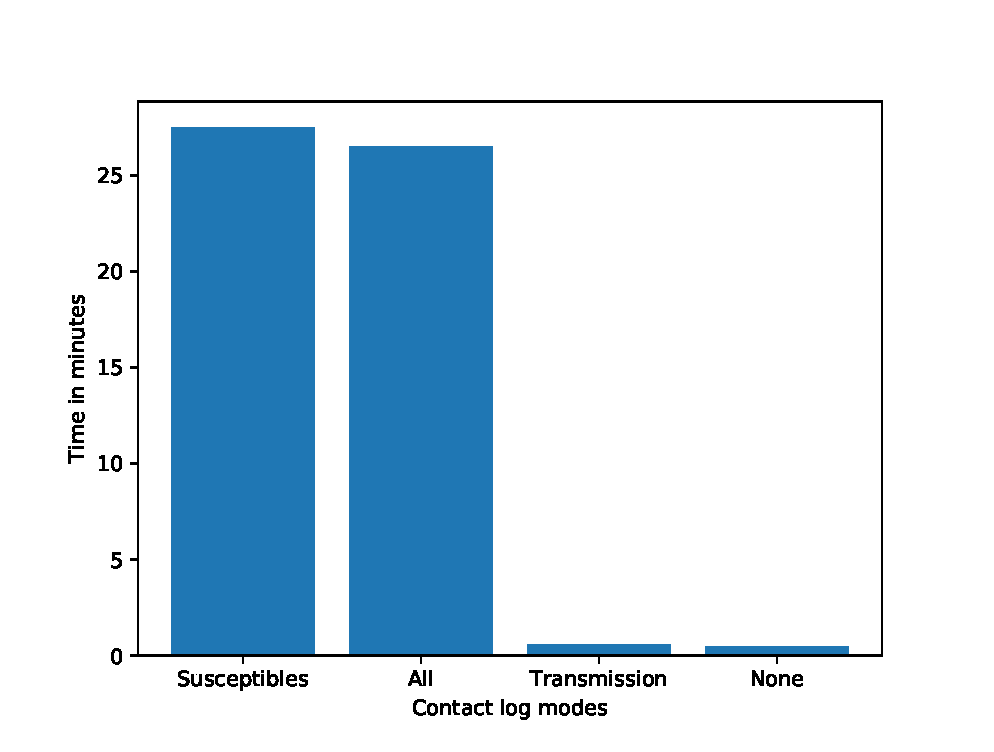
\includegraphics[width=0.8\textwidth]{3_GProf_contactlogmode.eps}
	\caption{Plot showing run time of simulations using different logging methods.} 
	\label{Gprof_contactlogmode}
\end{figure}

\end{document}
